\documentclass{article}
\usepackage{nips13submit_e,times}
\usepackage[utf8x]{inputenc}
\usepackage{amsfonts}
\usepackage{indentfirst}
\usepackage{hyperref}
\usepackage{graphicx}
\usepackage{enumerate}
\usepackage{amsmath}
\usepackage{subfigure} 
\usepackage{amsopn}
\title{Project-II by group TORONTO}
\author{Michalina Pacholska \And Jakub Sygnowski}
\nipsfinalcopy
\begin{document}
\maketitle
\begin{abstract}
This report describes our work on second project done for Machine Learning class at EPFL in Fall 2014. We were given...
\end{abstract}

\begin{figure}[!h]
\center
%\subfigure[Boxplot of original input data $\mathbf{X}$. Data is not centered and therefore we normalize it.]{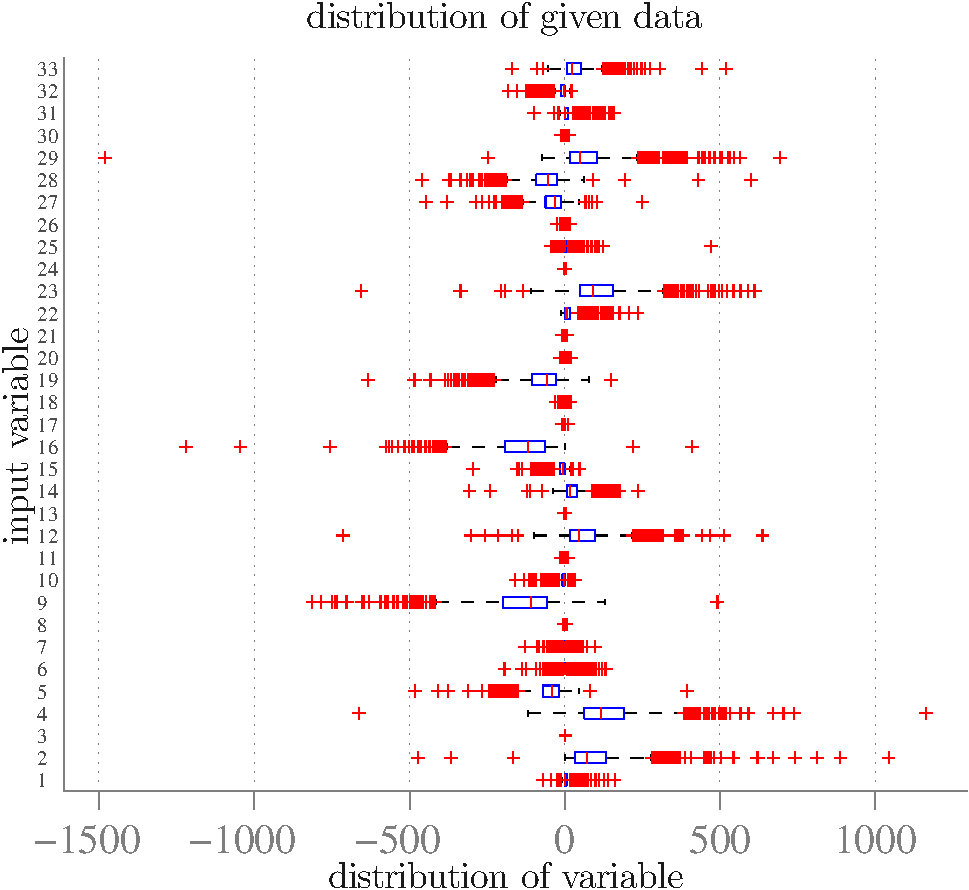
\includegraphics[width=2.5in]{../figures/classif/boxplot_before-crop.pdf} \label{fig:boxplotBefore}}
\hfill
%\subfigure[Boxplot of input data after normalization and removing outliers.]{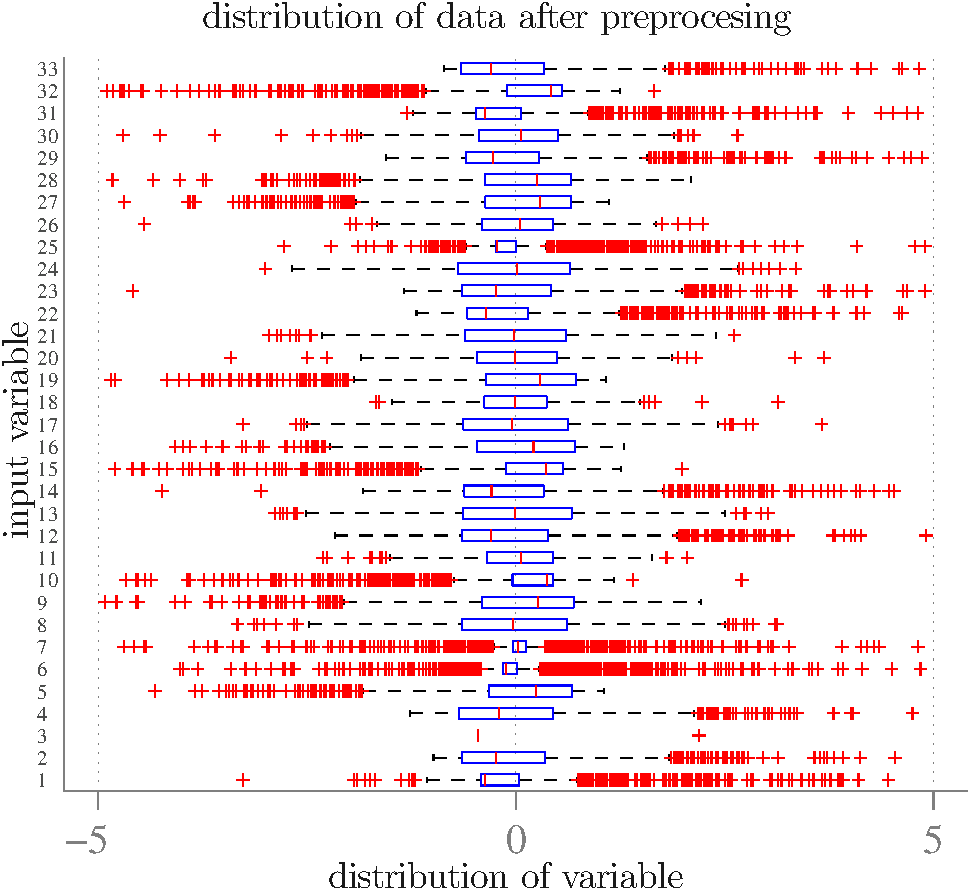
\includegraphics[width=2.5in]{../figures/classif/boxplot_after-crop.pdf} \label{fig:boxplotAfter}}
\caption{asdfasdf}
\end{figure}

\section*{Acknowledgments}

\end{document}
